\section{Stromrichter Schaltungen}


\subsection{Gruppierung nach Steuerung}
\begin{enumerate}
    \item \textbf{Ungesteuerter Stromrichter:} \\
    Bei ungesteuerten Stromrichtern ist das Verhältnis von Eingangs- zu Ausgangsspannung durch die Stromrichterschaltung festgesetzt.
    \item \textbf{Gesteuerter Stromrichter:} \\
    Bei steuerbaren Stromrichtern kann das Verhältnis von Eingangs- zu Ausgangsspannung durch den Steuereingriff am Halbleiterschalter verändert werden.
\end{enumerate}

\subsection{Gruppierung nach Führung}
\begin{enumerate}
    \item \textbf{Netzgeführte Schaltungen:}\\
    Die Kommutierungsspannung des Stromrichters wird von dem Netzwerk entnommen.
    \item \textbf{Lastgeführte Schaltungen:}\\
    Die Lastkreise (Synchronmotoren, Schwingkreise, usw.) liefern die Kommutierungsspannung.
    \item \textbf{Selbstgeführte Schaltungen:}\\
    Eigene Schaltmittel des Stromrichters erzeugen die Kommutierungsspannung.
\end{enumerate}

\subsection{Ungesteuerter Gleichrichter (M1U)}
\subsubsection{Ungesteuerter Gleichrichter (M1U) mit ohmscher Last}
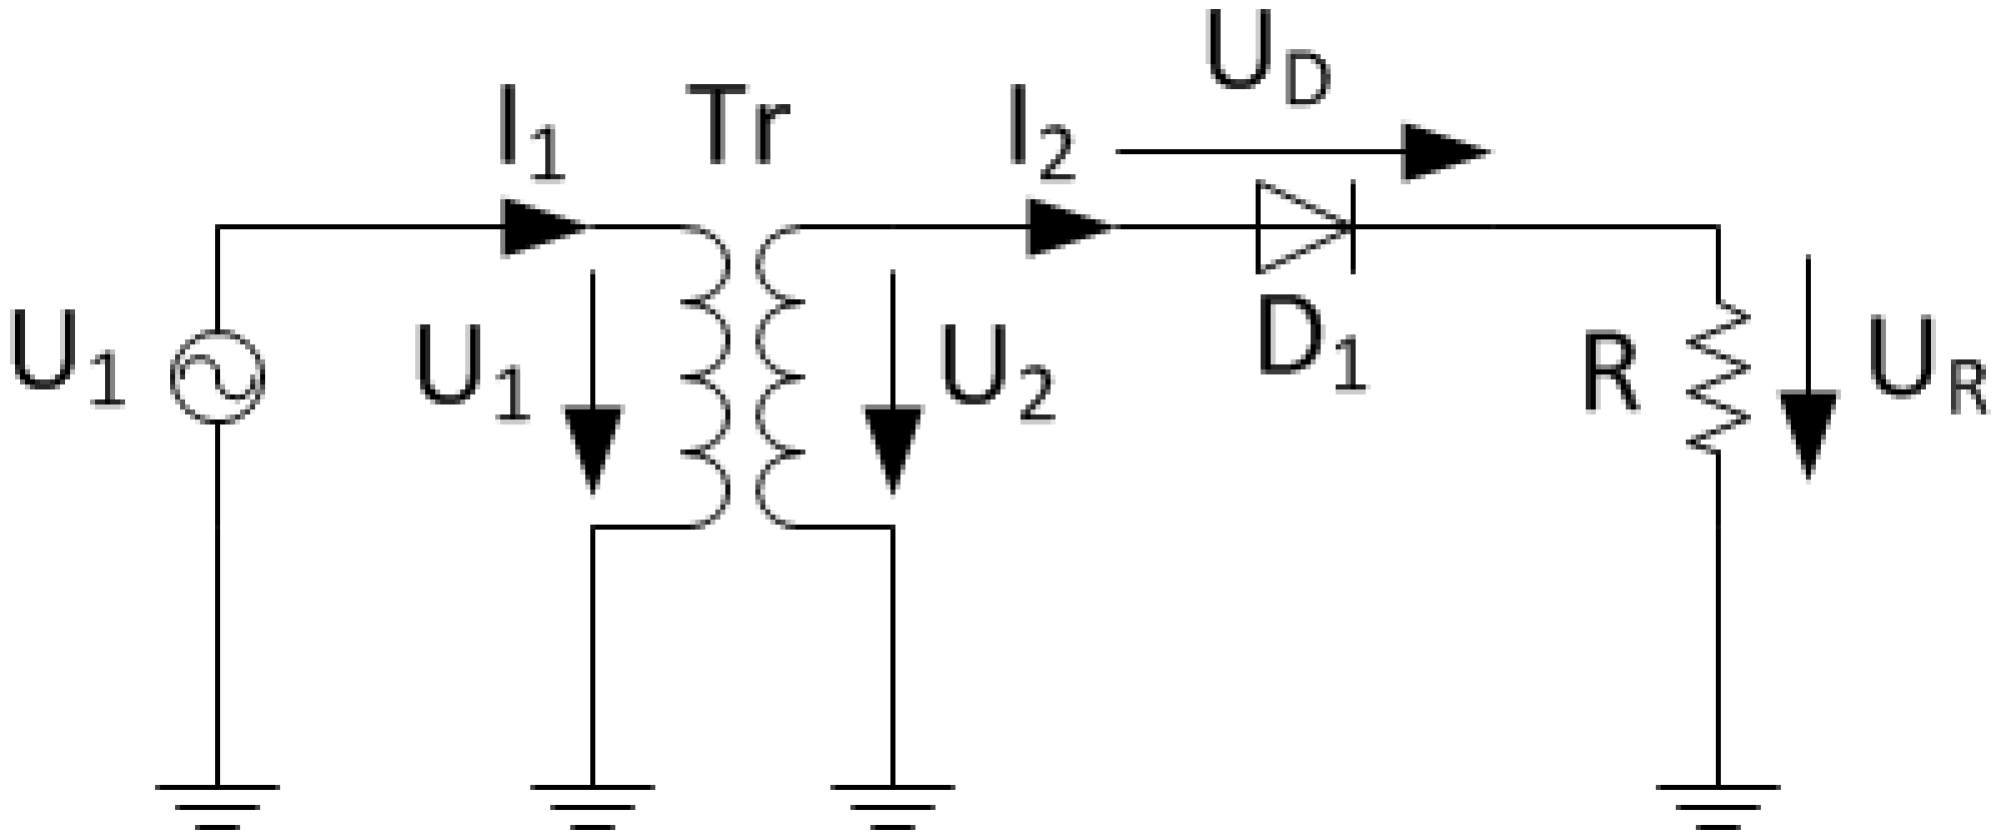
\includegraphics[width=0.8\columnwidth]{images/V3B02.png} \\

\textbf{Die Grundgleichungen:}

$
\boxed{U_2 = U_D + U_R}
$
$
\boxed{U_R = I_2 \cdot R}
$\\

\myul{In Durchlassrichtung:}\\
$
0 < \omega t < \pi \quad \quad U_R = U_2, \; U_D = 0
$\\
\myul{In Sperrrichtung}:\\
$
\pi < \omega t < 2\pi \quad \quad U_R = 0, \; U_D = U_2
$\\

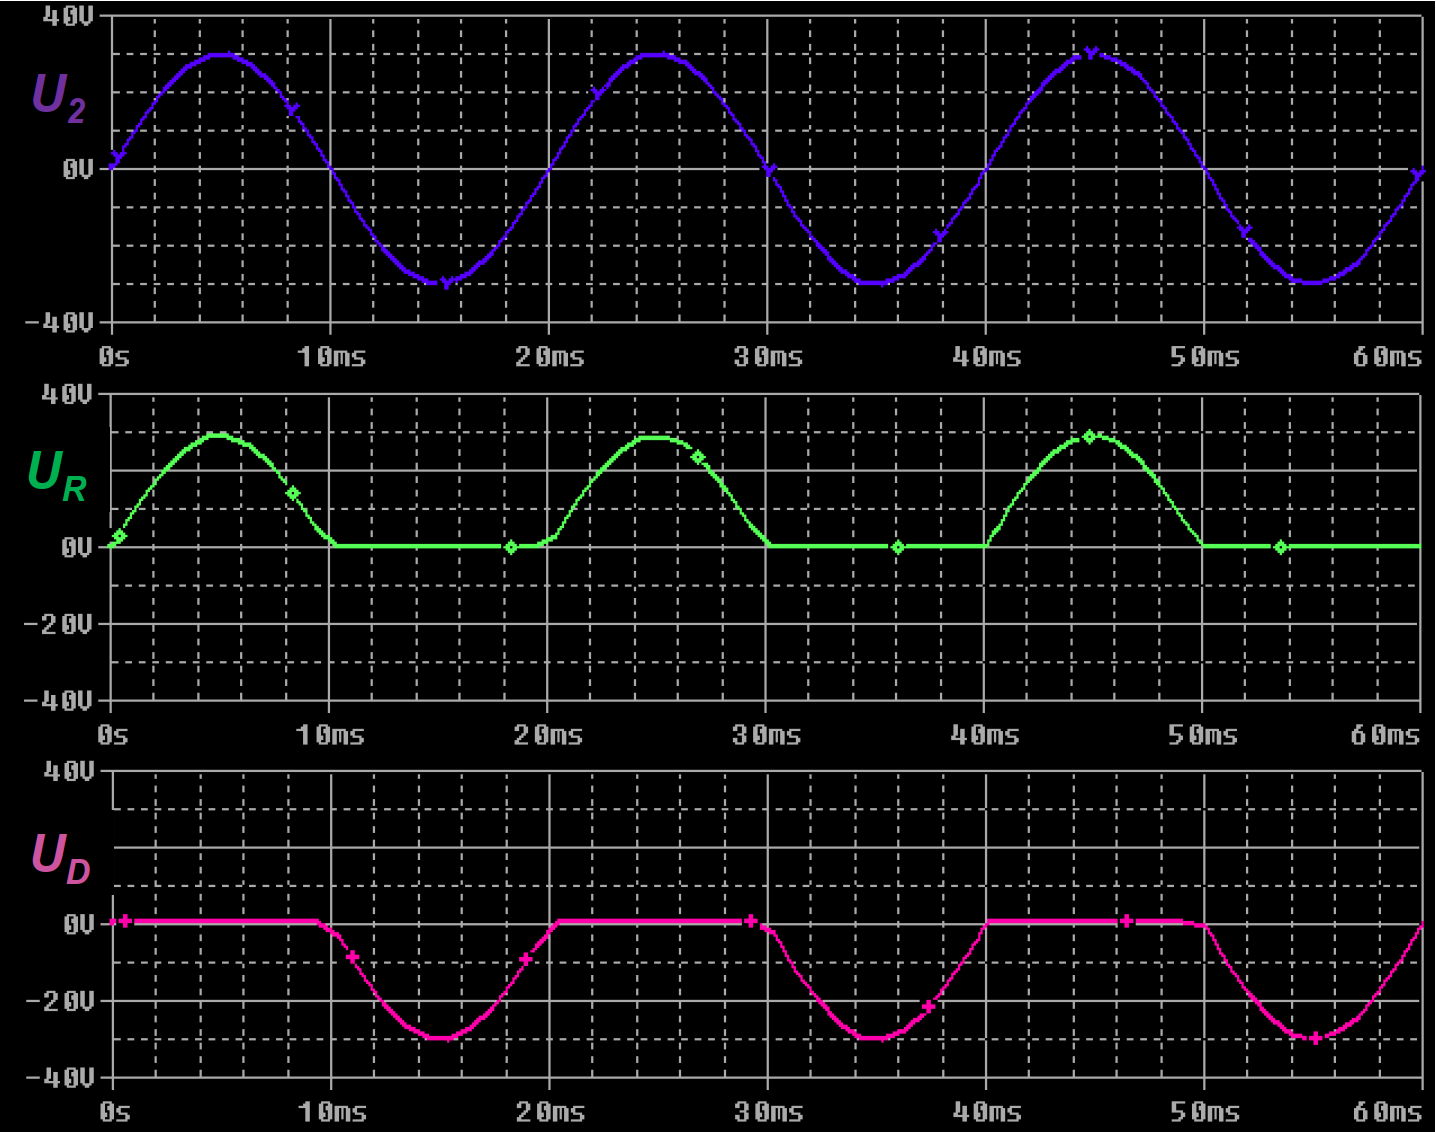
\includegraphics[width=0.8\columnwidth]{images/V3B03.png} \\

\myul{$U_{R_{AV}}$ Mittelwert der Spannung über der Last R}

$\boxed{U_{R_{AV}} 
= \frac{1}{T} \int_{0}^{T} u_R(t) \cdot dt 
= \frac{1}{2\pi} \int_{0}^{\pi} \hat{U}_{2} \cdot \sin(\alpha) \cdot d\alpha
= -\frac{\hat{U}_{2}}{2\pi} (\cos\pi - \cos0)
= \frac{\hat{U}_{2}}{\pi}}$\\
wobei gilt: $\alpha = \omega \cdot t$\\

\myul{$U_{R_{RMS}}$ Effektivwert der Spannung über der Last R}

$\boxed{
\begin{array}{lll}
    U_{R_{\text{RMS}}}  &=& \sqrt{\frac{1}{T} \int_{0}^{T} u_R^2(t) \cdot dt} \\
                        &=& \sqrt{\frac{1}{2\pi} \int_{0}^{\pi} \hat{U}_2^2 \cdot \sin^2(\alpha) \cdot d\alpha} \\
                        &=& \sqrt{\frac{\hat{U}_2^2}{2\pi} \int_{0}^{\pi} \sin^2(\alpha) \cdot d\alpha} \\
                        &=& \frac{\hat{U}_2}{2}
\end{array}}$\\

Hinweis: $\int_{0}^{\pi} \sin^2(\alpha) \cdot d\alpha = \frac{\pi}{2}$\\




